\chapter{Appendix}%
\label{chap:appendix}

\appendix

\textit{This intro to chapter appendix.\bs}
\todo[inline]{shortly introduce appendsix}

% \section{System Identification Methods}
% \subsection{Prediction Error Minimisation}
% \subsection{Prediction Error Minimisation}
%
% \section{Control Methods}
% \subsection{\acs{MPC}}
% \subsection{\acs{MPPI}}

\chapter{Complexity Classes}%
\label{chap:appendix_complexity_classes}
Problems in class P have a solution which can be found in polynomial time, problems in \ac{NP} are problems for which a solution cannot found in polynomial time. For problems in \ac{NP}, when provided with a solution, verifying that the solution is indeed a valid solution can be done in polynomial time. \ac{NP-hard} problems are a class of problems which are at least as hard as the hardest problems in \ac{NP}. Problems that are \ac{NP-hard} do not have to be elements of NP. They may not even be decidable~\cite{pokharel_computational_2020}. This thesis or other recent studies in the references do not attempt to find an optimal solution. Instead, they provide a solution whilst guaranteeing properties such as near-optimality or probabilistic completeness. We conclude that the \ac{NAMO} problem combined with relocating objects to target positions fall in the category of \ac{NP-hard} problems because it can be reduced to the piano's mover problem.\bs

\chapter{Control Methods}%
\label{chap:appendix_control_methods}

\section{\ac{MPC} Control}
\todo[inline]{Go over this section and update to the standart of the thesis, now that is clearly lit study}
In recent literature involving predictive methods \acf{MPC} methods are dominating, before moving on to \ac{MPC} and variations of \ac{MPC}, \ac{MPC} will briefly be explained.  The basic concept of \ac{MPC} is to use a dynamic model to forecast system behaviour and optimise the forecast to produce the best decision for the control move at the current time. Models are therefore central to every form of \ac{MPC}. Because the optimal control move depends on the initial state of the dynamic system~\cite{rawlings_model_2020}. A dynamical model can be presented in various forms, let's consider a familiar differential equation. 
$$ \frac{dx}{dt} = f(x(t), u(t)) $$
$$ y = h(x(t), u(t)) $$ 
$$ x(t_0) = x_0 $$

In which $x \in \mathbb{R}^n $ is the state, $u \in \mathbb{R}^m$ is the input, $y \in \mathbb{R}^p$ is the output, and $t \in \mathbb{R}$ is time. The initial condition specifies the value of the state $x$ at $t = t_0$, and a solution to the differential equation for time greater than $t_0$, $t \in \mathbb{R}_{\geq 0}$ is sought. If little knowledge about the internal structure of a system is available, it may be convenient to take another approach where the state is suppressed, no internal structure about the system is known and the focus lies only on the manipulable inputs and measurable outputs. As shown in \cref{figure: mpc_block_diagam}, consider the system $G(t)$ to be
the connection between $u$ and $y$. In this viewpoint, various system identification techniques are used, in which $u$ is manipulated and $y$ is measured~\cite{rawlings_model_2020}. From the input-output relation, a system model is estimated or improved. The system model can be seen inside the \ac{MPC} controller block in \cref{figure: mpc_block_diagam}.\\

\begin{figure}[h]
\centering
\begin{tikzpicture}
% blocks
\node[draw,
    minimum width=2cm,
    minimum height=1.2cm,
    fill=myLightColor,
] (system) at (0,0){$G(t)$};
\node[draw,
    minimum width=5.5cm,
    minimum height=2cm,
    fill=myEvenLighterColor,
    below = 1cm of system,
    label=above:MPC controller,
] (controller) {};
% the blocks and arrows inside MPC
\node[draw, minimum width=2cm, below=3mm of controller.north, anchor=north, fill=myDarkColor] (optimisation) {Optimisation};
\node[draw, below=8mm of optimisation.south, anchor=south, fill=myDarkColor] (model) {System Model};
\path[-stealth]
        (model.east) edge[bend right=70] node[pos=0.5, right] {Predict} (optimisation.east)
        (optimisation.west) edge[bend right=70] node[pos=0.5, left] {Action}  (model.west);
% Arrows
\draw[-stealth] (controller.west) |- ($(controller.west) - (1,0mm) $) |- (system.west) 
node[near end, above]{$u(t)$};
\draw[stealth-] ([yshift=-0.3cm]controller.east) -- ++(3,0) node[midway, above](input){$y_{ref}(t)$, $p$, $\mathbb{X}$, $\mathbb{U}$, $\mathbb{Y}$};
\draw[-stealth] (system.east) -- ++ (5, 0) 
    node[midway](output){}node[midway,above]{$y(t)$};
    \draw [-stealth] (output.center) |- ([yshift=0.5cm]controller.east); 
\end{tikzpicture}
\caption{System $G(t)$ with input ${u}(t)$, output $y(t)$ and \acs{MPC} controller with input $y(t)$, reference signal $y_{ref}(t)$, parameterisation $p$ and constraint sets $\mathbb{X}$, $\mathbb{U}$, $\mathbb{Y}$} \label{figure: mpc_block_diagam} \end{figure}  

As indicated in the problem description in TODO, prior knowledge about the structure of the robot itself is known. Such structure can be specified in a parameterisable system model, in which the influence of inputs and current states describes the behaviour of states and outputs. Uncertain parameters have to be sought, such as the center of mass, mass, and diameter of wheels. These parameters reside in the parameterisation $p$, see TODO. \Cref{figure: mpc_block_diagam} shows the parameterisation $p$, for purely analytical system models the parameterisation is left empty. The following explanation about \ac{MPC} is best understood with the differential drive robot in mind from TODO, with single-body model TODO. Some states of the system might be inside an obstacle region, such a region is undesirable for the robot to be in or go toward. The robot states are allowed in free space, which is all space minus the obstacle region. The free space is specified as a state constrained set $\mathbb{X}$. Allowable input can be restricted by the input constraint set $\mathbb{U}$, a scenario in which input constraints are required is for example the maximum torque an engine produces at full throttle. Lastly, the set of allowed outputs is specified in the output constraint set $\mathbb{Y}$. State, input and output constraints must be respected during optimisation, the optimiser takes the state-, input- and output constraint sets $\mathbb{X}$, $\mathbb{U}$, $\mathbb{Y}$ and if feasible, finds an action sequence driving the system toward the reference signal while constraints are respected. The \ac{MPC} system model predicts future states where the system is steered toward as a result of input actions.\\

The optimisation minimises an objective function $V_{N}(x_{0}, y_{ref}, \mathbf{u}_{N}(0))$, where\\ $ \mathbf{u}_{N}(k) = (u_k, u_{k+1}, \dots , u_{k+N})$. The objective function takes the reference signal as an argument together with the initial state and the control input for the control horizon. The objective function then creates a weighted sum of some heuristic function. States and inputs resulting in outputs far from the reference signal are penalised more by the heuristic function than outputs closer to the reference signal. Because the objective function is a Lyapunov function, it has the property that, it has a global minimum for the optimal input $\mathbf{u}_{N}^*$. If the system output reaches the reference signal $y_{ref}$, $x_{ref}$ then $u_{ref}$ will be mapped to the output reference signal as such $y_{ref} = h(x_{ref}, u_{ref})$. As a result solving the minimisation problem displayed in \cref{equation: mpc_problem} gives the optimal input which steers the system toward the output reference signal while at the same time respecting the constraints. 

\begin{mini}
{u_k, u_{k+1}, \dots , u_{k+N}} {
V_{N}(x_{0}, y_{ref}, u_k, u_{k+1}, \dots , u_{k+N})
}
{}{}
\addConstraint{x(k+1) = f(x(k), u(k))}
\addConstraint{x \in \mathbb{X}}
\addConstraint{u \in \mathbb{U}}
\addConstraint{y \in \mathbb{Y}}
\addConstraint{x(0) = x_0}
\label{equation: mpc_problem}
\end{mini}

\Cref{figure: mpc_scheme_basic} displays the predicted output converging toward the constant output reference. After solving the minimisation problem, \cref{equation: mpc_problem}, the optimal input sequence is obtained $\mathbf{u}^*_N$ (given that the constraints are respected for such input), from which only the first input is executed for time step $k$ to $k+1$. Then all indices are shifted such that the previous time step $k+1$ becomes $k$, the output is measured and the reference signal, parameterisation, and constraints sets are updated and a new minimisation problem is created, which completes the cycle. Note that \cref{figure: mpc_block_diagam,figure: mpc_scheme_basic} is an example \ac{MPC} controller, which hardly scratched the surface of \ac{MPC}, there are many variations and additions such as deterministic and stochastic \ac{MPC}, stage and terminal cost, distributed \ac{MPC}, etc. which~\cite{rawlings_model_2020} visits extensively. 

\begin{figure}[h]
    \centering
    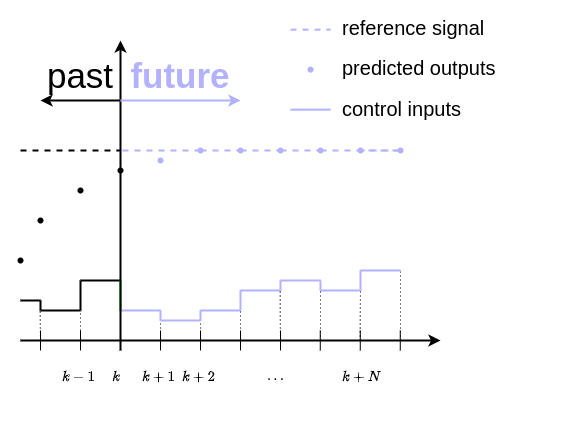
\includegraphics[width=0.8\textwidth]{figures/MPC_simple_diagram.png}
    \caption{A discrete \acs{MPC} scheme tracking a constant reference signal. $k$ indicates the discrete time step, $N$ the control horizon}
    \label{figure: mpc_scheme_basic}
\end{figure}

A major flaw for \ac{MPC} was the computation time required to solve a minimisation problem every time step. Because processors' power has increased, the \ac{MPC} framework can be applied in real time and is applicable for robotics. When applied to tracking a reference signal the \ac{MPC} framework outperforms classic control approaches such as PID control~\cite{nascimento_nonholonomic_2018}. Where \ac{MPC} excels at is tracking multiple objectives which can be weighted in the objective function. For example, \ac{MPC} can primarily track a robot path, while secondarily satisfying some additional dynamic specifications. This makes \ac{MPC} especially suitable in path tracking for nonholonomic robots. By restricting the state constraint set, obstacles can be avoided, such obstacles can even be avoided online  because the state constraint set may be changed during execution. It should however be feasible to find an input which satisfies all constraints. Because of its ease of tuning, handling multiple objectives, and flexibility in adding constraints, \ac{MPC} became the baseline standard to compare new control approaches with in control research. By now, linear \ac{MPC} theory is quite mature, and important issues
such as stability are well addressed in the last decade. Nevertheless, some systems are, in general,
inherently nonlinear. Therefore, especially in highly dynamic systems such as mobile robotics, linear
models are often inadequate to describe the process dynamics and nonlinear models have to be used. Thus nonlinear \ac{MPC} theory is required for which closed-loop stability proofs are lacking~\cite{nascimento_nonholonomic_2018}. \\


\section{\ac{MPPI} Control}
\todo[inline]{Go over this section and update to the standart of the thesis, now that is clearly lit study}
Introduced by~\cite{williams_model_2015} \ac{MPPI} control arose. Which was followed by \ac{MPPI} control combined with various system models, identification methods~\cite{abraham_modelbased_2020,cong_selfadapting_2020,arruda_uncertainty_2017}. The core idea is from the current state of the system with the use of a system model and randomly sampled inputs to simulate in the future a number of "rollouts" for a specific time horizon,~\cite{neuromorphictutorial_ltc21_2021}. These rollouts indicate the future states of the system if the randomly sampled inputs would be applied to the system, the future states can be evaluated by a cost function which penalised undesired states and rewards desired future states. A weighted sum over all rollouts determines the input which will be applied to the system. If a goal state is not reached, the control loop starts with the next iteration. An example is provided, see  \cref{figure: mppi_car_with_rollouts}. 

\begin{figure}[h]
    \centering
    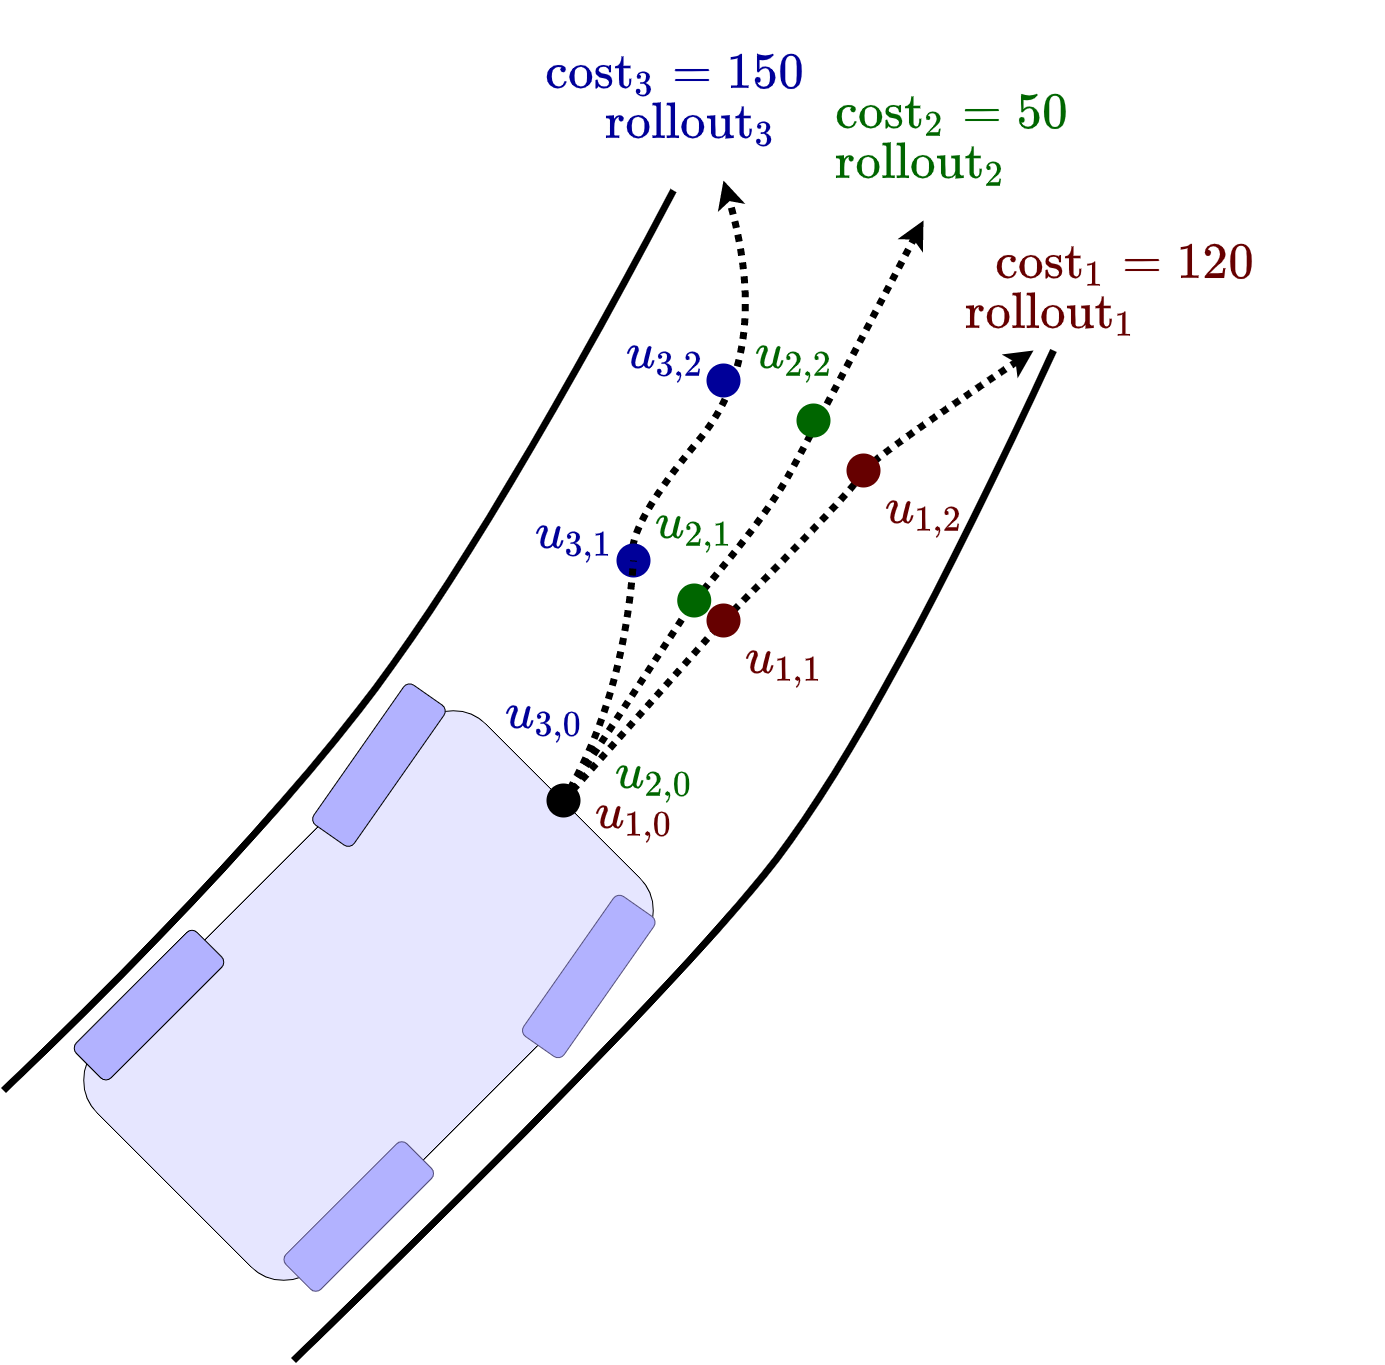
\includegraphics[width=0.5\textwidth]{figures/MPPI_car_with_rollouts.png}
    \caption{\acs{MPPI} controlled race car using a control horizon of 3 time steps, with 3 rollouts all having their respected inputs as $u_{i,j}$ where $i$ is the rollout index and $j$ indicates the time step~\cite{neuromorphictutorial_ltc21_2021}.}
    \label{figure: mppi_car_with_rollouts}
\end{figure}

Here 3 rollouts are displayed, The objective function is designed to keep the car driving on the center of the road by penalising rollouts which are further away from the center of the road relatively more. resulting in a high cost for $\text{rollout}_1$ and $\text{rollout}_3$ compared to $\text{rollout}_2$. As a result, the input send to the system as a weighted sum of the rollouts is mostly determined by $\text{rollout}_2$. The weighted sum determining the input is displayed in \cref{equation: mppi_weighted_sum}, from~\cite{neuromorphictutorial_ltc21_2021}.

\begin{equation}
u(k+1)=u(k)+\frac{\sum_{i} w_{i} \delta u_{i}}{\sum_{i} w_{i}}
\label{equation: mppi_weighted_sum}
\end{equation}

Where $\delta u_i$ is the difference between $u(k)$ and the input for rollout $i$, the weight of $\text{rollout}_i$ is detemined as: $w_{i}=e^{-\frac{1}{\lambda} \text{cost}_{i}}$, $\lambda$ is a constant parameter. The reader is now somewhat familiar with the \ac{MPPI} concept, Now some applications with \ac{MPPI} and multi-object control are discussed.\bs

\chapter{Implementation in Python}%
\label{chap:code_implementation}


Code reproducibility in the scientific community is low~\cite{trisovic_largescale_2022}. That is bad, bad bad bad!

\todo[inline]{setup of the system (python version, ubuntu version etc.)}
\todo[inline]{reference to an install readme file}
\todo[inline]{Explain what can be changed easily}
\todo[inline]{Explain code folders (the thingies better to not touch)}
\todo[inline]{Explain code folders (the thingies better to not touch)}
\todo[inline]{What should be done again}
